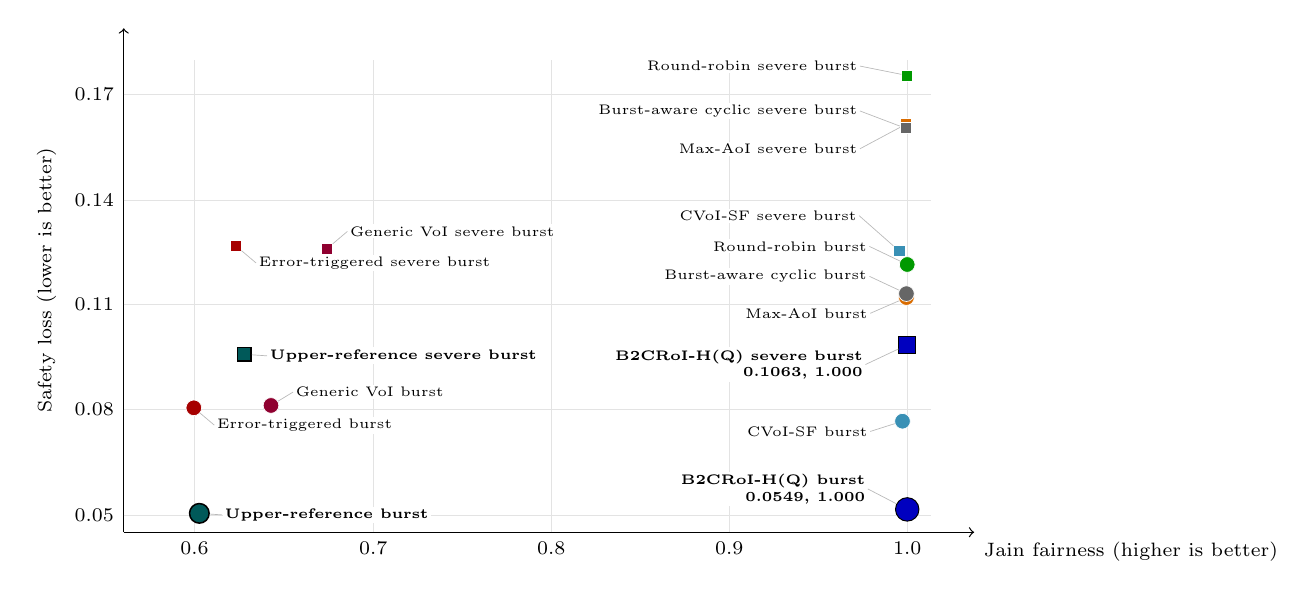
\begin{tikzpicture}[font=\scriptsize]
% Labelled Pareto summary. Axes are scaled from fairness in [0.6, 1.0]
% and safety loss in [0.05, 0.18]. Each plotted unit is labelled directly.
\draw[->,line width=0.45pt] (0,0) -- (10.8,0) node[below right]{Jain fairness (higher is better)};
\draw[->,line width=0.45pt] (0,0) -- (0,6.4);
\node[rotate=90] at (-0.98,3.2) {Safety loss (lower is better)};

% Grid and ticks.
\foreach \x/\lab in {0.90/0.6,3.17/0.7,5.43/0.8,7.69/0.9,9.95/1.0}{
  \draw[gray!22,line width=0.25pt] (\x,0) -- (\x,6.0);
  \node[below] at (\x,0) {\lab};
}
\foreach \y/\lab in {0.22/0.05,1.56/0.08,2.89/0.11,4.22/0.14,5.56/0.17}{
  \draw[gray!22,line width=0.25pt] (0,\y) -- (10.25,\y);
  \node[left] at (0,\y) {\lab};
}

\tikzset{
  burst/.style={circle,draw=white,line width=0.25pt,inner sep=2.0pt},
  severe/.style={rectangle,draw=white,line width=0.25pt,inner sep=2.0pt},
  proposed/.style={fill=blue!75!black,draw=black,line width=0.35pt,inner sep=3.0pt},
  upperref/.style={fill=teal!70!black,draw=black,line width=0.55pt,inner sep=2.5pt},
  err/.style={fill=red!65!black}, voi/.style={fill=purple!75!black},
  cvoi/.style={fill=cyan!70!black}, maxaoi/.style={fill=orange!85!black},
  cyc/.style={fill=gray!80!black}, rr/.style={fill=green!60!black},
  lab/.style={font=\tiny,fill=white,inner sep=0.8pt,align=left},
  call/.style={gray!55,line width=0.25pt}
}

% Burst points and labels.
\node[burst,proposed] (b2b) at (9.95,0.29) {};
\node[lab,anchor=east,font=\bfseries\tiny,align=right] (b2bl) at (9.45,0.55) {B2CRoI-H(Q) burst\\0.0549, 1.000};
\draw[call] (b2bl.east) -- (b2b);
\node[burst,upperref] (urb) at (0.96,0.24) {};
\node[lab,anchor=west,font=\bfseries\tiny] (urbl) at (1.25,0.22) {Upper-reference burst};
\draw[call] (urbl.west) -- (urb);
\node[burst,err] (eb) at (0.89,1.58) {};
\node[lab,anchor=west] (ebl) at (1.15,1.36) {Error-triggered burst};
\draw[call] (ebl.west) -- (eb);
\node[burst,voi] (vb) at (1.87,1.61) {};
\node[lab,anchor=west] (vbl) at (2.15,1.78) {Generic VoI burst};
\draw[call] (vbl.west) -- (vb);
\node[burst,cvoi] (cb) at (9.89,1.41) {};
\node[lab,anchor=east,align=right] (cbl) at (9.48,1.28) {CVoI-SF burst};
\draw[call] (cbl.east) -- (cb);
\node[burst,maxaoi] (ab) at (9.94,2.98) {};
\node[lab,anchor=east,align=right] (abl) at (9.48,2.78) {Max-AoI burst};
\draw[call] (abl.east) -- (ab);
\node[burst,cyc] (gb) at (9.94,3.03) {};
\node[lab,anchor=east,align=right] (gbl) at (9.47,3.25) {Burst-aware cyclic burst};
\draw[call] (gbl.east) -- (gb);
\node[burst,rr] (rb) at (9.95,3.40) {};
\node[lab,anchor=east,align=right] (rbl) at (9.47,3.63) {Round-robin burst};
\draw[call] (rbl.east) -- (rb);

% Severe-burst points and labels.
\node[severe,proposed] (b2s) at (9.95,2.38) {};
\node[lab,anchor=east,font=\bfseries\tiny,align=right] (b2sl) at (9.42,2.13) {B2CRoI-H(Q) severe burst\\0.1063, 1.000};
\draw[call] (b2sl.east) -- (b2s);
\node[severe,upperref] (urs) at (1.53,2.26) {};
\node[lab,anchor=west,font=\bfseries\tiny] (ursl) at (1.82,2.24) {Upper-reference severe burst};
\draw[call] (ursl.west) -- (urs);
\node[severe,err] (es) at (1.42,3.64) {};
\node[lab,anchor=west] (esl) at (1.68,3.42) {Error-triggered severe burst};
\draw[call] (esl.west) -- (es);
\node[severe,voi] (vs) at (2.58,3.60) {};
\node[lab,anchor=west] (vsl) at (2.84,3.82) {Generic VoI severe burst};
\draw[call] (vsl.west) -- (vs);
\node[severe,cvoi] (cs) at (9.85,3.57) {};
\node[lab,anchor=east,align=right] (csl) at (9.34,4.02) {CVoI-SF severe burst};
\draw[call] (csl.east) -- (cs);
\node[severe,maxaoi] (as) at (9.93,5.18) {};
\node[lab,anchor=east,align=right] (asl) at (9.35,4.87) {Max-AoI severe burst};
\draw[call] (asl.east) -- (as);
\node[severe,cyc] (gs) at (9.93,5.13) {};
\node[lab,anchor=east,align=right] (gsl) at (9.35,5.35) {Burst-aware cyclic severe burst};
\draw[call] (gsl.east) -- (gs);
\node[severe,rr] (rs) at (9.95,5.80) {};
\node[lab,anchor=east,align=right] (rsl) at (9.35,5.92) {Round-robin severe burst};
\draw[call] (rsl.east) -- (rs);
\end{tikzpicture}
